\documentclass[12pt, twoside]{article}
\usepackage[letterpaper, margin=1in, headsep=0.5in]{geometry}
\usepackage[english]{babel}
\usepackage[utf8]{inputenc}
\usepackage{amsmath}
\usepackage{amsfonts}
\usepackage{amssymb}
\usepackage{tikz}
\usetikzlibrary{quotes, angles}
\usepackage{graphicx}
%\usepackage{pgfplots}
%\pgfplotsset{width=10cm,compat=1.9}
%\usepgfplotslibrary{statistics}
%\usepackage{pgfplotstable}
%\usepackage{tkz-fct}
%\usepackage{venndiagram}

\usepackage{fancyhdr}
\pagestyle{fancy}
\fancyhf{}
\renewcommand{\headrulewidth}{0pt} % disable the underline of the header

\fancyhead[RE]{\thepage}
\fancyhead[RO]{\thepage \\ Name: \hspace{3cm}}
\fancyhead[L]{BECA / Dr. Huson / Geometry 10th Grade\\* Unit 2: Midpoints and distance \\ 
18 September 2019}

\begin{document}
  \subsubsection*{2.3 Do Now: Midpoint calculations \& rectangle measurements}
    \begin{enumerate}

    \item Given $\overleftrightarrow{TC}$ as shown on the number line. \\[20pt] % Midpoint
    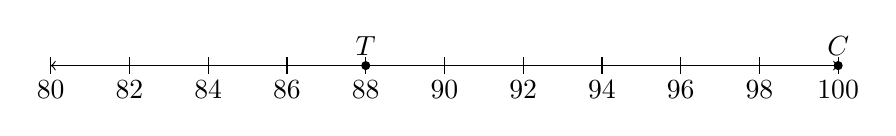
\begin{tikzpicture}[scale=0.5]
      \draw [<->] (80,0)--(100,0);
      \foreach \x in {80, 82,...,100} %2 leading for diff!=1
        \draw[shift={(\x,0)},color=black] (0pt,-6pt) -- (0pt,6pt) node[below=5pt]  {$\x$};
        \draw [fill] (88,0) circle [radius=0.1] node[above] {$T$};
        \draw [fill] (100,0) circle [radius=0.1] node[above] {$C$};
    \end{tikzpicture} \\ \bigskip
    What is the midpoint between the points $T$ and $C$? \vspace{2cm}  

    \item Find the measure of $\angle P$ in degrees? \vspace{0.25cm}
    %\begin{enumerate}
      %\item  $m \angle GEF = $ \rule{4cm}{0.15mm} \bigskip
      %\item  $EG=$ \rule{4cm}{0.15mm} \bigskip
      %\item Name a pair of opposite rays: \rule{4cm}{0.15mm} \bigskip
    %\end{enumerate}
    \begin{center}
    \begin{tikzpicture}[scale=1]
      \draw [->, thick] (0,0)--(140:5);
      \draw [->, thick] (0,0)--(20:7);
      %\draw [->, thick] (0,0)--(-1.2,3);
      %\draw [fill] (-1,2.5) circle [radius=0.05] node[left ]{$B$};
      %\draw [fill] (35:3) circle [radius=0.05] node[above left ]{$G$};
      %\draw [fill] (-2,0) circle [radius=0.05] node[below]{$D$};
      \draw [fill] (0,0) circle [radius=0.05] node[below]{$P$};
      %\draw [fill] (4,0) circle [radius=0.05] node[above]{$F$};
    \end{tikzpicture}
    \end{center}  \vspace{1cm}

    \item Given $\overline{AMB}$, $M$ bisects $\overline{AB}$, $AM=3x-10$, $BM=x+4$. Find ${AB}$.\\
    Complete all the steps for full credit. \smallskip
      \begin{enumerate}
        \item Sketch and label the situation
        \item Write an equation
        \item Solve for $x$
        \item Answer the question
        \item Check your solution
      \end{enumerate}

 \newpage
    \item Draw a rectangle that is 9 centimeters long horizontally and 4 centimeters tall vertically. (use a square to ensure the sides are perpendicular)  \vspace{6cm}

    \item Given the rectangle $ABCD$ shown below, with $AB=10$ and $BC=5$. The diagonal $\overline{AC}$ is drawn to create two triangles. Find the area of the lower triangle, $\triangle ABC$.
    \begin{flushleft}
    \begin{tikzpicture}
      \draw [-, thick] (0,0)--(10,0)--(10,5)--(0,5)--cycle;
      \draw [-, thick] (0,0)--(10,5);
      \draw [fill] (0,0) circle [radius=0.05] node[left]{$A$};
      \draw [fill] (10,0) circle [radius=0.05] node[right]{$B$};
      \draw [fill] (10,5) circle [radius=0.05] node[right]{$C$};
      \draw [fill] (0,5) circle [radius=0.05] node[left]{$D$};
      \node at (10.5, 2.5){5};
      \node at (5, -0.5){10};
    \end{tikzpicture}
    \end{flushleft}
    \vspace{3cm}

    \item The line segment $\overline{MN}$ is trisected by the points $K$ and $L$. Given that $MN=15$. \\ Find $KL$. (draw a picture)

\end{enumerate}
\end{document}


\item Given line segment $\overline{AB}$ with midpoint $M$, that is, $\overline{AM} \cong \overline{BM}$. $AB=11.8$. Find the length of $\overline{AM}$.\\[0.75cm]
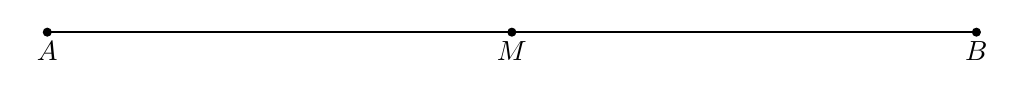
\begin{tikzpicture}
  \draw [-, thick] (0,0)--(11.8,0);
  \draw [fill] (0,0) circle [radius=0.05] node[below]{$A$};
  \draw [fill] (11.8,0) circle [radius=0.05] node[below]{$B$};
  \draw [fill] (5.9,0) circle [radius=0.05] node[below]{$M$};
\end{tikzpicture}
\vspace{3cm}
